%%%%%%%%%%%%%%%%%%%%%%%%%%%%%%%%%%%%%%%%%
% Beamer Presentation
% LaTeX Template
% Version 1.0 (10/11/12)
%
% This template has been downloaded from:
% http://www.LaTeXTemplates.com
%
% License:
% CC BY-NC-SA 3.0 (http://creativecommons.org/licenses/by-nc-sa/3.0/)
%
%%%%%%%%%%%%%%%%%%%%%%%%%%%%%%%%%%%%%%%%%

%----------------------------------------------------------------------------------------
%	PACKAGES AND THEMES
%----------------------------------------------------------------------------------------

\documentclass{beamer}

\mode<presentation> {

% The Beamer class comes with a number of default slide themes
% which change the colors and layouts of slides. Below this is a list
% of all the themes, uncomment each in turn to see what they look like.

%\usetheme{default}
%\usetheme{AnnArbor}
%\usetheme{Antibes}
%\usetheme{Bergen}
%\usetheme{Berkeley}
%\usetheme{Berlin}
%\usetheme{Boadilla}
%\usetheme{CambridgeUS}
%\usetheme{Copenhagen}
%\usetheme{Darmstadt}
%\usetheme{Dresden}
%\usetheme{Frankfurt}
%\usetheme{Goettingen}
%\usetheme{Hannover}
%\usetheme{Ilmenau}
%\usetheme{JuanLesPins}
%\usetheme{Luebeck}
\usetheme{Madrid}
%\usetheme{Malmoe}
%\usetheme{Marburg}
%\usetheme{Montpellier}
%\usetheme{PaloAlto}
%\usetheme{Pittsburgh}
%\usetheme{Rochester}
%\usetheme{Singapore}
%\usetheme{Szeged}
%\usetheme{Warsaw}

% As well as themes, the Beamer class has a number of color themes
% for any slide theme. Uncomment each of these in turn to see how it
% changes the colors of your current slide theme.

%\usecolortheme{albatross}
%\usecolortheme{beaver}
%\usecolortheme{beetle}
%\usecolortheme{crane}
%\usecolortheme{dolphin}
%\usecolortheme{dove}
%\usecolortheme{fly}
%\usecolortheme{lily}
%\usecolortheme{orchid}
%\usecolortheme{rose}
%\usecolortheme{seagull}
%\usecolortheme{seahorse}
%\usecolortheme{whale}
%\usecolortheme{wolverine}

%\setbeamertemplate{footline} % To remove the footer line in all slides uncomment this line
%\setbeamertemplate{footline}[page number] % To replace the footer line in all slides with a simple slide count uncomment this line

%\setbeamertemplate{navigation symbols}{} % To remove the navigation symbols from the bottom of all slides uncomment this line
}

\usepackage{graphicx} % Allows including images
\usepackage{booktabs} % Allows the use of \toprule, \midrule and \bottomrule in tables
\usepackage{multirow}
\usepackage{adjustbox}
\usepackage{array}
\usepackage{tikz}
\usepackage{soul}
\usepackage{pdfpages}
\usetikzlibrary{shapes.geometric, arrows, positioning, fit}
\usepackage[latin1]{inputenc}
\newcommand{\xmark}{\textcolor{red}{\text{\sffamily X}}}
\newcommand{\cmark}{\textcolor{green}{\checkmark}}
\newcommand{\tr}{\text{tr}}
\newcommand{\E}{\textbf{E}}
\newcommand{\diag}{\text{diag}}
\newcommand{\argmax}{\text{argmax}}
\newcommand{\argmin}{\text{argmin}}
\newcommand{\Cov}{\text{Cov}}
\newcommand{\Var}{\text{Var}}
\newcommand{\Vol}{\text{Vol}}
\newcommand{\bx}{\boldsymbol{x}}
\newcommand{\by}{\boldsymbol{y}}
\newcommand{\bX}{\boldsymbol{X}}
\newcommand{\bY}{\boldsymbol{Y}}
\sethlcolor{gray}
\makeatletter
\newcommand\SoulColor{%
  \let\set@color\beamerorig@set@color
  \let\reset@color\beamerorig@reset@color}
\makeatother
\definecolor{color1}{RGB}{128,13,13}
\definecolor{color2}{RGB}{70,128,13}
\definecolor{color3}{RGB}{13,128,128}
\definecolor{color4}{RGB}{70,13,128}

%tikz stufff


%----------------------------------------------------------------------------------------
%	TITLE PAGE
%----------------------------------------------------------------------------------------


\title[JSM 2017]{Cool things from JSM 2017}

\author{Charles Zheng} % Your name
\institute[NIMH] % Your institution as it will appear on the bottom of every slide, may be shorthand to save space
{National Institute of Mental Health}
\date{\today} % Date, can be changed to a custom date

\begin{document}

\begin{frame}
\titlepage % Print the title page as the first slide
\end{frame}

\begin{frame}
\frametitle{Inference without assumptions}
\begin{itemize}
\item Larry Wasserman, ``Inference without assumptions, Review and Current Progress''
\item Conformal prediction by Vovk, Gammerman and Shafer (2006) \pause
\item Exact prediction intervals, \emph{only} needing to assume i.i.d. data
\begin{itemize}
\item Suppose $Y_1,\hdots, Y_n \sim F$ iid
\item Construct set $S$, such that
\[
\Pr[Y^* \in S] \geq 1 -\alpha
\]
for a new $Y^* \sim F$.
\end{itemize}
\pause
\item Application to $k$-means..
\end{itemize}
\end{frame}

\begin{frame}
\frametitle{Using conformal prediction to choose $k$}
\begin{center}
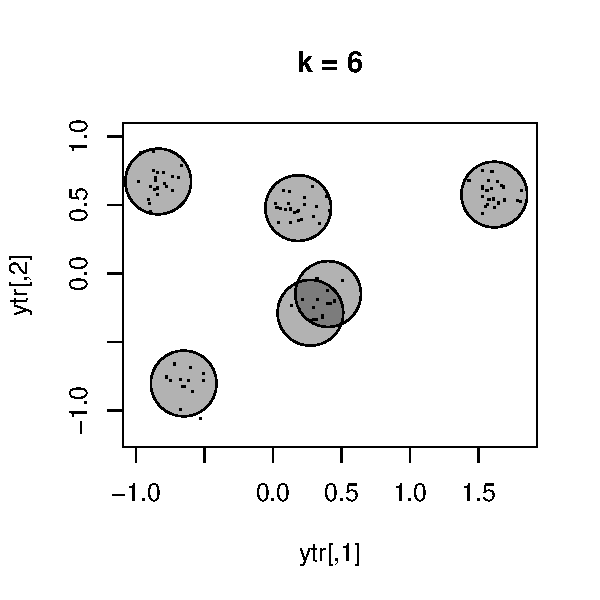
\includegraphics[scale = 0.3, clip = true, trim = 0.3in 0.4in 0.3in 0.2in]{../conformal_kmeans/k6.pdf}
\end{center}
\begin{itemize}
\item Wasserman's idea: build prediction set using $k$-means and data-splitting. \pause
\item Resulting prediction set is a union of spheres $S$ centered around the centroids, with the propoerty that
\[
\Pr[Y^* \in S] \geq 1 -\alpha
\]
for a new point $Y^*$ \pause
\item When spheres intersect, merge those clusters.\pause
\end{itemize}
Does it work?  I tried it out myself..
\end{frame}

\begin{frame}
\frametitle{Simple simulation with $k=5$ and $\alpha = 0.05$}
\newcommand{\scalesize}{0.3}
\begin{center}
\begin{tabular}{ccc}
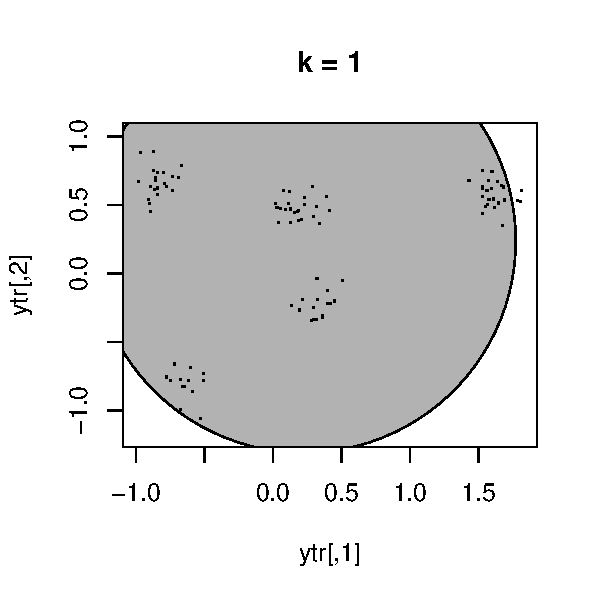
\includegraphics[scale = \scalesize, clip = true, trim = 0.3in 0.4in 0.3in 0.2in]{../conformal_kmeans/k1.pdf} &
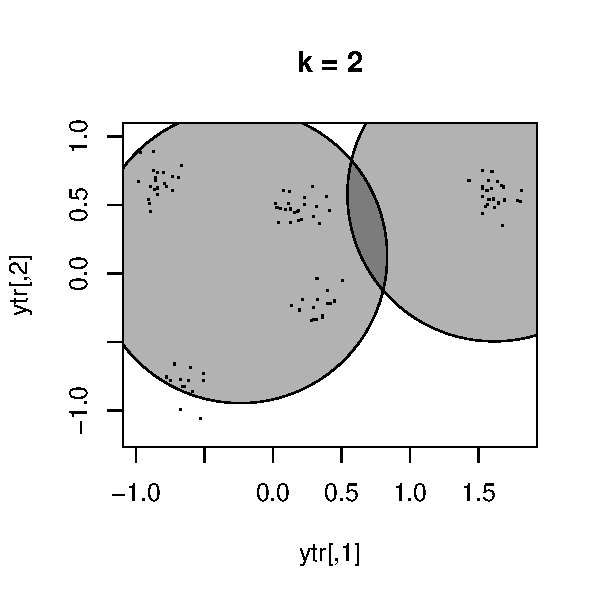
\includegraphics[scale = \scalesize, clip = true, trim = 0.3in 0.4in 0.3in 0.2in]{../conformal_kmeans/k2.pdf} &
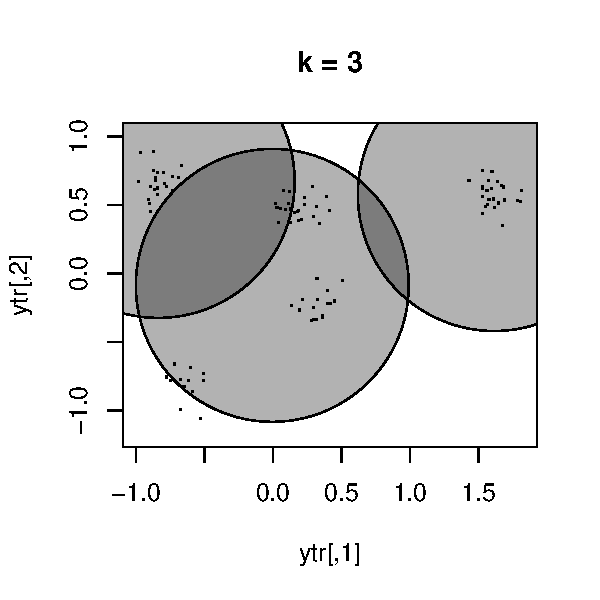
\includegraphics[scale = \scalesize, clip = true, trim = 0.3in 0.4in 0.3in 0.2in]{../conformal_kmeans/k3.pdf} \\
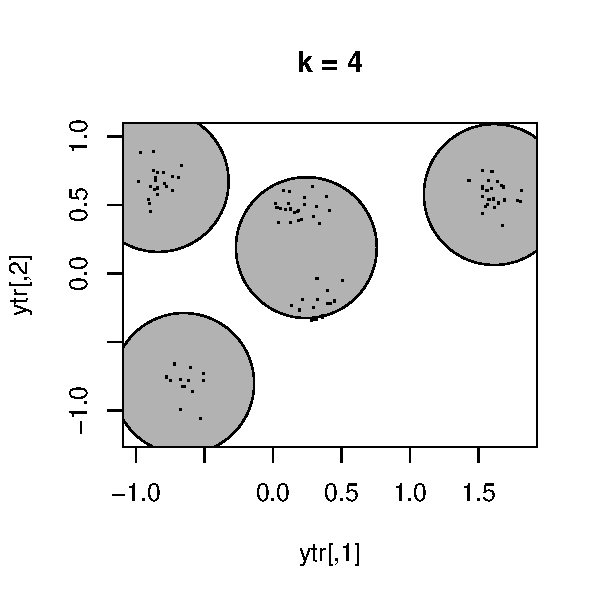
\includegraphics[scale = \scalesize, clip = true, trim = 0.3in 0.4in 0.3in 0.2in]{../conformal_kmeans/k4.pdf} &
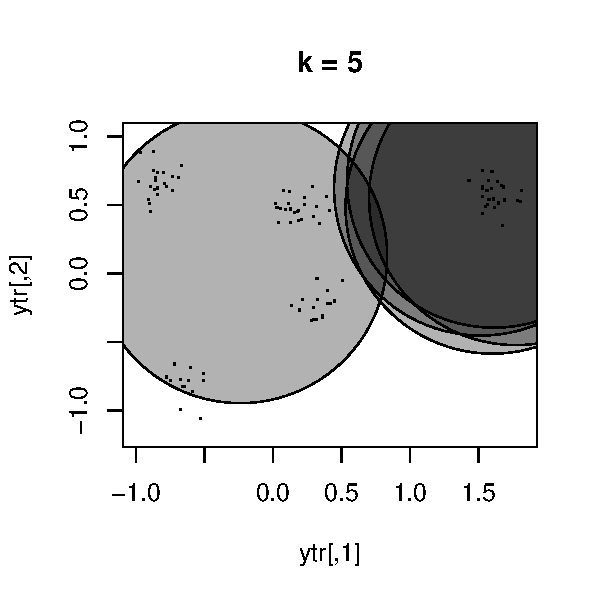
\includegraphics[scale = \scalesize, clip = true, trim = 0.3in 0.4in 0.3in 0.2in]{../conformal_kmeans/k5.pdf} &
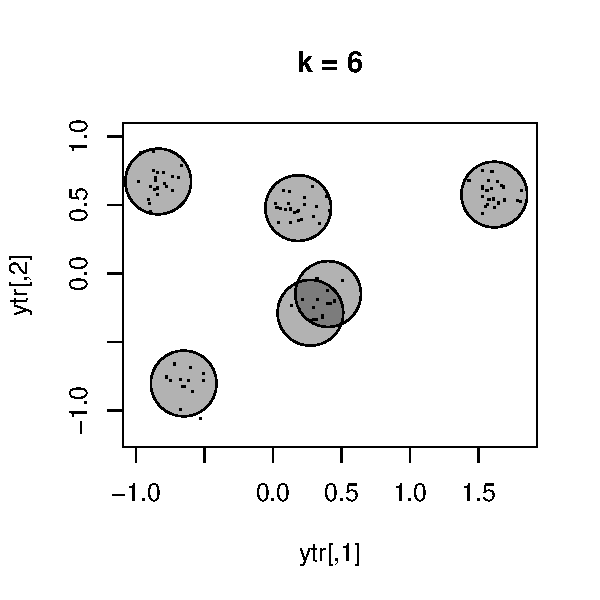
\includegraphics[scale = \scalesize, clip = true, trim = 0.3in 0.4in 0.3in 0.2in]{../conformal_kmeans/k6.pdf} \\
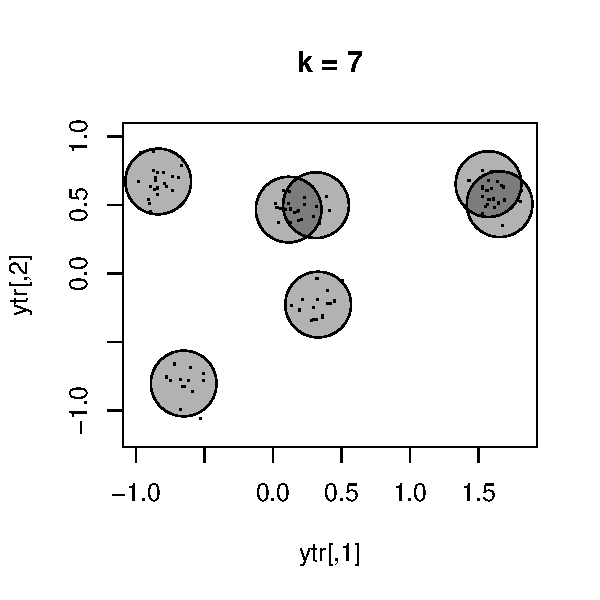
\includegraphics[scale = \scalesize, clip = true, trim = 0.3in 0.4in 0.3in 0.2in]{../conformal_kmeans/k7.pdf} &
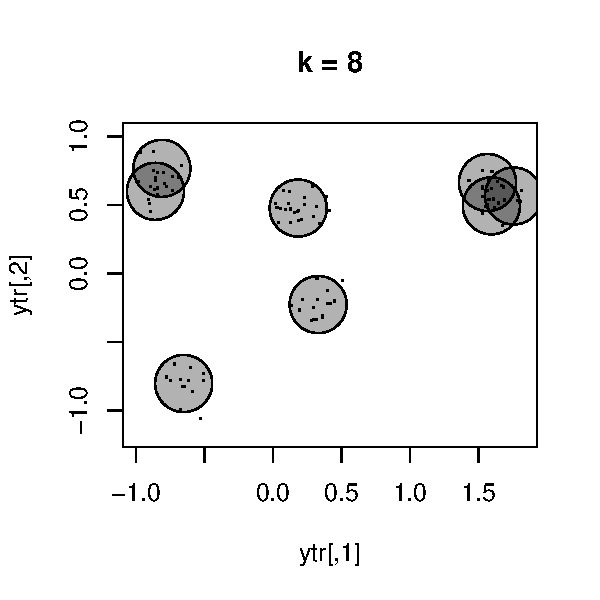
\includegraphics[scale = \scalesize, clip = true, trim = 0.3in 0.4in 0.3in 0.2in]{../conformal_kmeans/k8.pdf} &
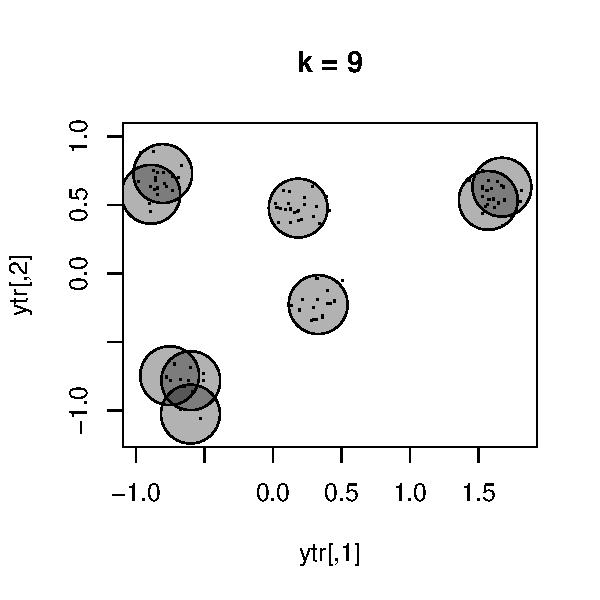
\includegraphics[scale = \scalesize, clip = true, trim = 0.3in 0.4in 0.3in 0.2in]{../conformal_kmeans/k9.pdf} \\
\end{tabular}
\end{center}
\end{frame}


\begin{frame}
\frametitle{JIVE-Joint and individual variation explained}
\begin{itemize}
\item Method for integrating two datasets, and decomposing into joint and individual variance components
\begin{center}
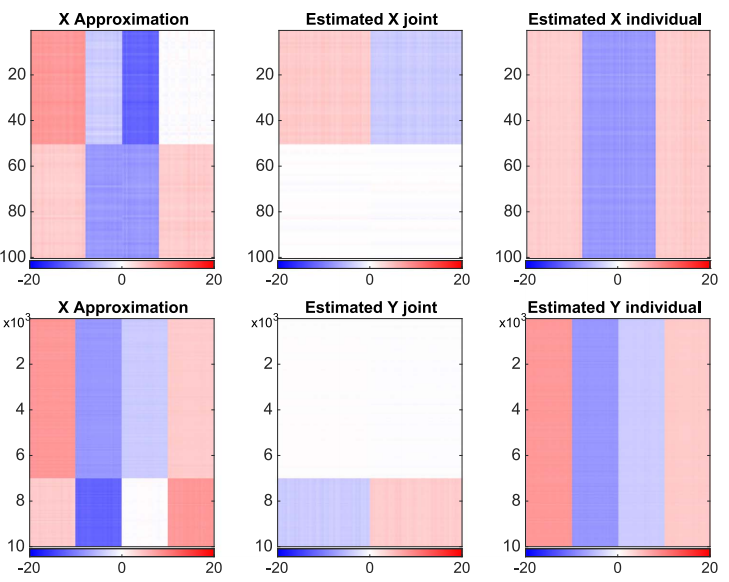
\includegraphics[scale = 0.25]{jsm_figs/jive_decomposition.png}
\end{center}
\item Angled-Based JIVE described in Feng, Hannig, Jiang and Marron (2017)
\end{itemize}
\end{frame}

\begin{frame}
\frametitle{JIVE-Joint and individual variation explained}
\begin{itemize}
\item Benjamin Risk described his joint work with Yu, Zhang and Marron applied to HCP data, comparing JIVE to PLS (partial least squares)
\begin{center}
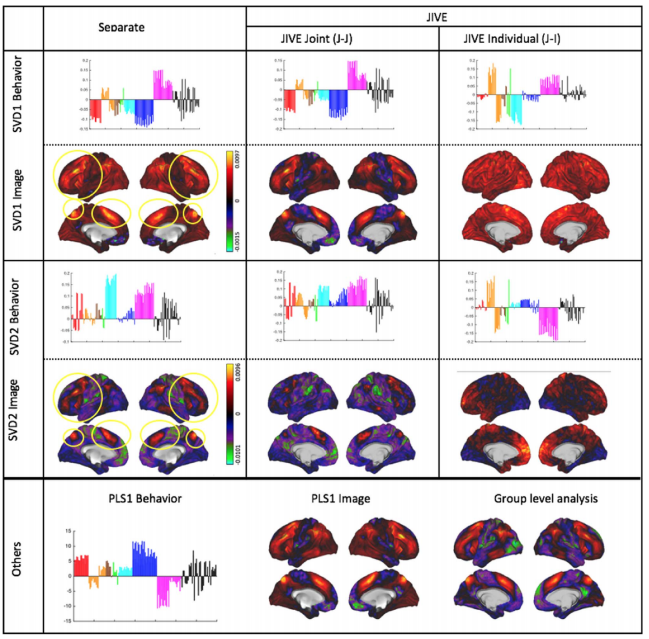
\includegraphics[scale = 0.3]{jsm_figs/jive_brain.png}
\end{center}
\end{itemize}
\end{frame}

\begin{frame}
\frametitle{Fingerprinting}
\begin{center}

\includegraphics[scale = 0.3]{jsm_figs/finngerprinting.png}


\includegraphics[scale = 0.3]{jsm_figs/airan_factors.png}
\end{center}
Brian Caffo is thinking about ``fingerprinting'' from a statistical point of view
\end{frame}

\end{document}
